%Statistics gathered during operation.
%Graphs, numbers, etc. Explain your results! What
%do your measurements show/mean?
\section{Statistics}
This section describes the statistics gathered from Exim, patterns we
found in those statistics, and what conclusions we can gather from that
data.

\begin{wrapfigure}{r}{0.6\textwidth}
  \vspace{-30pt}
  \begin{center}
    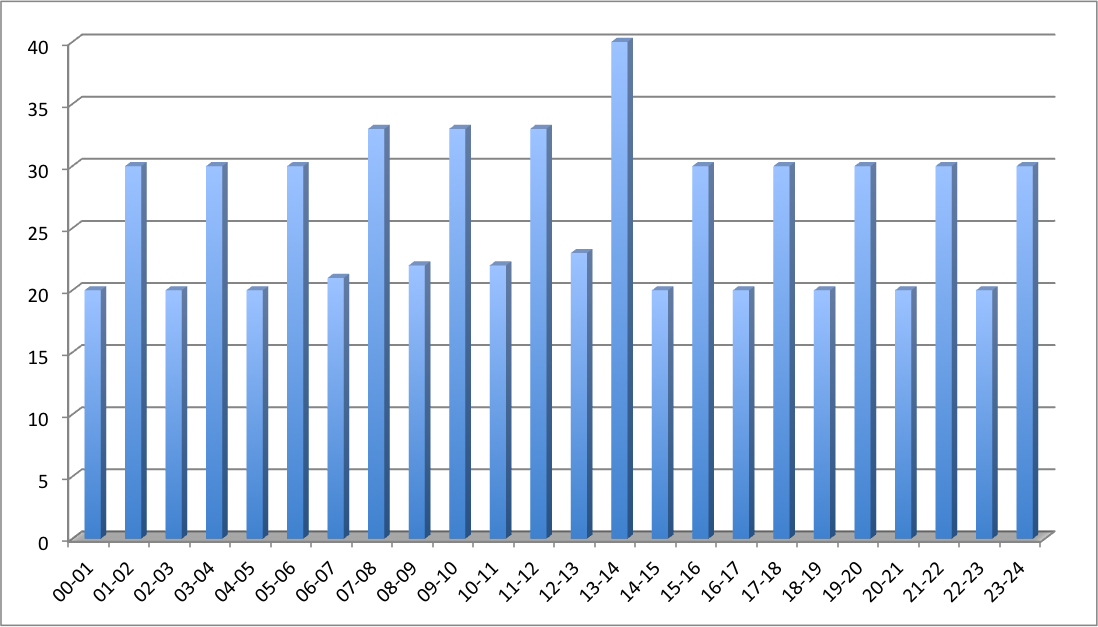
\includegraphics[scale=0.5]{img/per-hour.png}
  \end{center}
  \vspace{-20pt}
  \caption{\bf{Email per hour of each day}}
  \label{fig:mailperhour}
  \hspace*{20pt}
\end{wrapfigure}

Exim records all statistics regarding it operation in the logfiles
located in \emph{/var/log/mainlog}. Exim has a built in tool to gather
those statistics, namely \emph{eximstats}.\\\\
Figure~\ref{fig:mailperhour}  describes the amount of email processed (sent
and received) during the different hours of the days. This is highly
relevant in order to pick a good time for maintenance. However, as is
visible from the table, a email server that is always active is
difficult to maintain without interrupting the users. The reason for
this is a periodic script sending mail to the OS-group, we believe.
\begin{figure}[htb]
  \begin{center}
    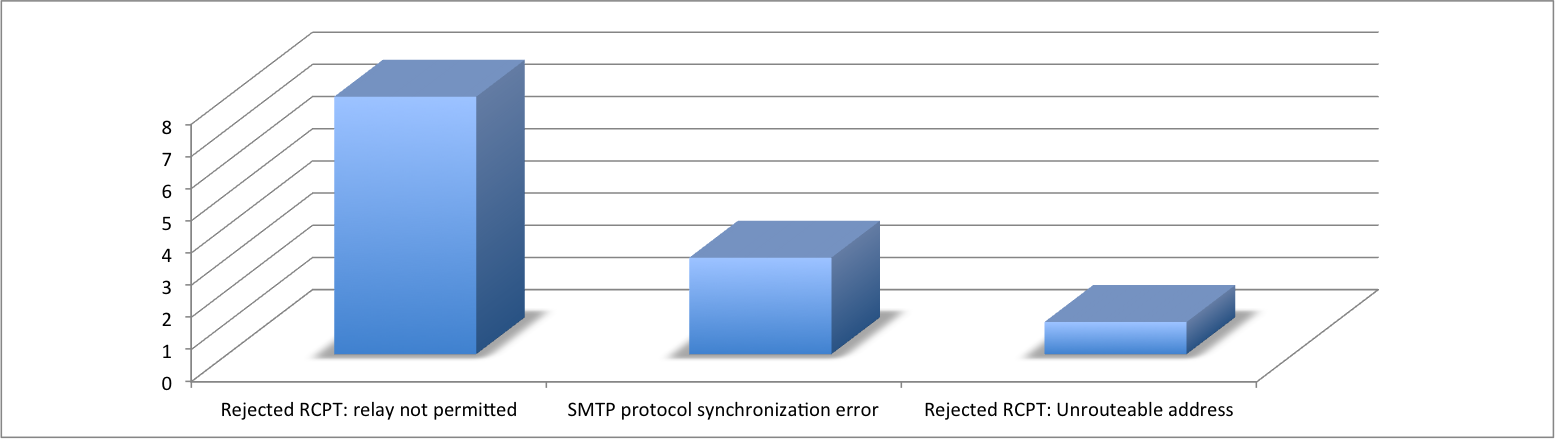
\includegraphics[scale=0.55]{img/rejection-reasons.png}
  \end{center}
  \caption{\bf{Reasons for rejection}}
  \label{fig:rejection}
\end{figure}
As an operator it's interesting to know why a particular email did not
reach it's destination. Figure~\ref{fig:rejection} describes the
different reasons for rejection and lists how many individual emails
that were the reason for these rejections. As we can derive from the
figure, a total of 8 mails were rejected due to relay permissions. We
believe the cause of this is misconfiguration of one or more
IMAP-clients. Below is the descriptions of the different rejection
reasons:
\begin{description}
\item \textbf{Rejected RCPT: relay not permitted} error means that someone tried to relay mail
using our SMTP server, which is not permitted. This can be caused by someone
using an email-client and using our SMTP server as an outgoing SMTP server
which, according to the SLA, is not permitted.

\item \textbf{SMTP protocol synchronization} error means that something or someone tried to
talk to our SMTP server using a non-spec SMTP protocol implementation. This can
be caused by someone manually telneting to our SMTP server and mess about with
it, or a faulty implementation.

\item \textbf{Rejected RCPT: Unrouteable address} means that the server could find the
specified address, and therefore, could not deliver the email. This error can be
avoided if you want by specifying that all unroutable mail should go to a
specified address, more often than not root@example.com. 

\end{description}
\begin{figure}[h!]
%  \vspace{-20pt}
  \begin{center}
    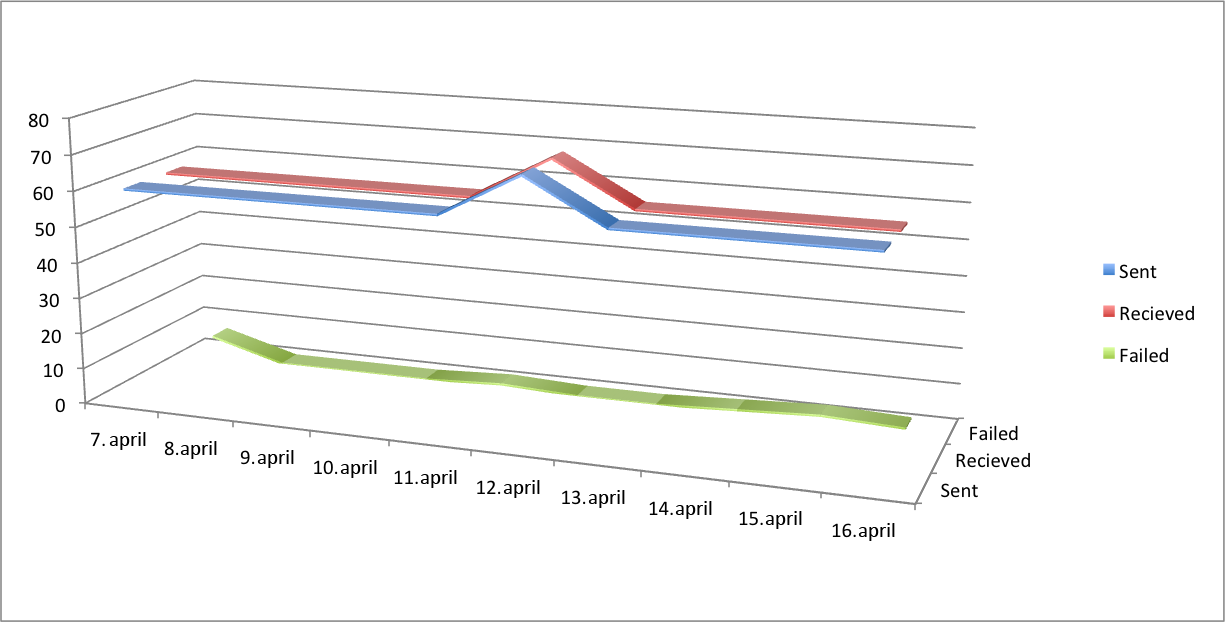
\includegraphics[scale=0.70]{img/sent-received-failed.png}
  \end{center}
 % \vspace{-20pt}
  \caption{\bf{Amount of email per day}}
  \label{fig:amount}
\end{figure}
Figure~\ref{fig:amount} describes the amount of email per day. From the
straight and coherent lines showing the sent and received statistics we
can deduct that all mail was probably sent and received by the same
server, i.e. the users of this particular email system were only
contacting eachother. The error rate is stable and fairly close to
zero.\newline
